%\documentclass[a4paper]{article}
\documentclass[10pt,a4paper]{article}
\usepackage[utf8]{inputenc} % para poder usar tildes en archivos UTF-8
\usepackage[spanish]{babel}
\usepackage{verbatim}
\usepackage{clrscode3e}

% \usepackage{bibtex}

%\usepackage{a4wide} % márgenes un poco más anchos que lo usual

\usepackage{caratula} % Se puede descargar en ~> https://github.com/bcardiff/dc-tex
\usepackage[breaklinks=true]{hyperref}


\begin{document} % Todo lo que escribamos a partir de aca va a aparecer en el documento.

%fran
%\sloppy

% Completar los datos de la caratula
\titulo{Trabajo Práctico 1 - Page Rank} 
\fecha{\today}
\materia{Métodos Numéricos}
\grupo{Grupo "Nombre Del Grupo"}

% Completar los integrantes del grupo:)
\integrante{Facundo, Araujo}{321/15}{facalj\_velez@hotmail.com}
\integrante{Cristian, Kubrak}{456/15}{Kubrakcristian@gmail.com}
\integrante{Marcela Alejandra, Herrera}{1162/84}{marcelaalejandraherrera@yahoo.com.ar}
\integrante{Luis Fernando, Greco}{150/15}{luifergreco@gmail.com}


\maketitle

% Aca comienzan a escribir su informe
\tableofcontents

\newpage

\section{Introducción}
\subsubsection*{Introducción Teórica}

\par El problema que se nos plantea es el de implementar un Page Rank, es decir, un método para ordernar páginas de acceso público de forma sistematizada y eficiente. Para esto tendremos que definir que parametros vamos a tener en cuenta al momento de armar nuestro órden de páginas. Estos van a ser, la cantidad de links "entrantes" a una página y la "calidad" de cada uno de estos (es decir, que tan relevante es la página de la que proviene ese link).\newline

\par Encontramos que este problema tiene una gran aplicación, dado que es fundamental para construir un motor de búsqueda y nos permitirá entender mejor como funcionan.\newline

\par HABLAR ALGO SOBRE CADENAS DE MARKOV


\par Para empezar al trabajar con matrices ralas nos vimos en la necesidad de buscar un método implementar este tipo de estructura, teniendo en cuenta un uso eficiente de los recursos del sistema (intentando sacar provecho del conocimiento que tenemos de entrada sobre las matrices). Es en este contexto que decidimos utilizar el formato CSR (Compressed Sparse Row), que vamos a proceder a explicar detalladamente más adelante.\newline

\par 
\newpage

% \section{Demostraciones}
% \newpage

\section{Desarrollo}

\par Las relaciones entre p\'aginas forman un grafo y resulta conveniente almacenarlos como una
matriz de uno y ceros, done el un uno en la poscici\'on $ij$ representa que la p\'agina $j$ apunta a la $i$.
A\'un as\'i esta implementaci\'ion tiene un problema: debe almacenar $n^2$ elementos, donde solo importan
$m$ (la cantidad de unos). En la pr\'actica, $m \ll n^2$ (ya que no todas las p\'aginas se relacionan
con todos). Es por esto que decidimos utilizar matrices \textit{ralas}: un tipo de matriz donde solo
importa donde hay unos, es decir, qu\'e p\'agina apunta a cu\'al.
\par Como primer acercamiento, evaluamos utilizar dos conocidos conocidos m\'etodos para el almacenamiento
de matrices ralas: CSR (Compressed Sparse Row) y CSC (Compressed Sparse Column). En el primer caso
nos encotramos con el problema de la dificultad de acceder a las colmunas, mientras que en el segundo,
las filas. consideramos de vital importancia poder acceder tanto a filas como columnas en un tiempo
razonable para operaciones tales como la multiplicación o la Eliminación Gausseana.
\par Luego de evaluar los requerimientos, tanto de complejidad como de espacio utilizado, optamos
por implementar una estructura h\'ibrida entre un DOK (Dictionary Of Keys) y una lista de listas. 
Utilizamos una estructura que consiste en un diccionario de diccionarios: en el primero almacenamos
todas las filas y en el segundo sus elementos.
\par Respecto a la implementaci\'on, nos encontramos frente a la decisión de utilizar un diccionario ordenado
implementado sobre una estructura autobalanceada (\verb|std::map|) o un diccionario desordenado
implementado sobre una tabla de hash (\verb|std::unordered_map|). Si bien este \'ulitmo permite
el acceso en $O(1)$ en promedio frente al acceso en $O(\log n)$ del diccionario ordenado, 
no resulta f\'acil iterar eficientemete por lo que terminamos decidi\'endonos por la versi\'on autobalanceada.
\par Nuestro objectivo es resolver el listem a \ref{eq:Axx} o equivalentemente el sistema \ref{ipwd}, para lo cual 
resulta pr\'actico y eficiente utilizar Eliminación Gausseana:

\begin{codebox}
\Procname{$\proc{Eliminación Gausseana}(A)$}
\li \For $k \gets 1$ \To $n-1$
    \Do
\li     \For $i \gets k+1$ \To $n$
            \Do
\li         \For $j \gets k+1$ \To $n$
                \Do
\li                 $a_{ij} \gets a_{ij} - a_{ik}a_{kj}$
                \End
            \End
        \End
\end{codebox}

\par Como la matriz que utlizamos para almacenar la informci\'on es rala (no todos los elementos se encuentran definidos) por lo que 
adem\'as hay que asegurarse que los elementos est\'en definidos antes de operar con ellos. M\'as a\'un, dado que la resoluci\'on
del sistema no es m\'as que una aproximaci\'on, es necesario definir un $\varepsilon > 0$ para determinar qu\'e tan bien queremos que 
aproxime a la soluci\'on real; si bien un $\varepsilon$ m\'as chico producir\'ia una mejor aproximaci\'on, tambi\'en ralentiza la
ejecuci\'on del algoritmo. Es por esto, que junto con la esparsidad ($\delta = 1 - \frac{m}{n^2}$), decidimos hacer un an\'alisis
sobre el taman\~no del $\varepsilon$ por lo que el algoritmo de resoluci\'on queda:

\begin{codebox}\label{elimGaussRala}
\Procname{$\proc{Eliminación Gausseana Rala}(A)$}
\li \For $k \gets 1$ \To $n-1$
    \Do
\li     \For $i \gets k+1$ \To $n$
            \Do
\li         \For $j \gets k+1$ \To $n$
                \Do
\li                \If $a_{ik}.definido()$ and $a_{kj}.definido()$
                        \Then
\li                        $mult \gets a_{ik}/a_{kk}$
\li                     \If $a_{ij}.definido()$
                            \Then
\li                          $a_{ij} \gets a_{ij} - mult*a_{kj}$
\li                     \Else
\li                          $a_{ij} \gets - mult*a_{kj}$
                \End
            \End
        \End
\end{codebox}
Observar que en ning\'un momento verificamos que $a_{kk}$ est\'e definido ya que la matriz permite hacer Eliminación Gausseana sin necesidad
de pivoteo. (ver ap\'endice)
Luego para determinar las soluciones del sistema\cite{burden}:
\[
    x_n = \frac{a_{n,n-1}}{a_{nn}}
    \]
    \[
    x_i = \frac {a_{i,n+1} - \sum_{j=i+1}^{n} a_{ij}x} {a_{ii}}
    \]

Por \'ulitmo, normalizamos el vector $x$ de manera que $\sum^{n}_{i=1} |x_i| = 1$
\subsection*{Experimentaci\'on}
\par
En cuanto a la experimentaci\'on, pensamos en probar nuestra implementaci\'on de dos formas diferentes: de manera cualitativa y cuantitiativa.
Para realizar el an\'alisis cuantitativo, generamos matrices aleatorias para luego variar los distintos parametros tales como probabilidad, 
tamaño de la matriz, cantidad de links y epsilon, para poder luego evaluar su incidencia. Para el an\'alisis cualitativo, construimos casos particulares
que nos resultaron interesantes analizar por diversos motivos.

\par 

Con respecto al an\'alisis cuantitativo, variamos los tres par\'ametros que considerados que podr\'ian ser interesantes de analizar:
el tama\~no de la matriz $n$, la cantidad de links $m$, la probabilidad $p$ y el $\varepsilon$.
\newline
En el primero de estos tests, creamos matrices de entrada aleatorias con tamaño $n$, probabilidad $p$ y $\varepsilon$ fijos, mientras variaban la cantidad de links $m$
de la matriz generada, es decir cambiando qu\'e tan rala es. A partir de esto, buscamos encontrar una relaci\'on entre la \textit{sparsity} y el tiempo.\newline
En este test nuestra expectativa fue encontrarnos con un incremento en el tiempo a medida 
que la \textit{sparsity} de nuestra matriz de entrada era menor, considerando que la
implementaci\'on fue diseñada para funcionar de manera eficiente en matrices de este tipo.

\par
Como segundo test, buscamos evaluar incidencia del par\'ametro $p$ en el tiempo de ejecuci\'on en una matriz de tamaño $m$, cantidad de links $n$ 
y $\varepsilon$ fijos.\newline
Al ver la ecuaci\'on \ref{ipwd} observamos que a medida que el par\'ametro $p$ decrece, tambi\'en lo hace el resultado de $pWD$ y, 
por la forma en que implementamos la igualdad, tener elementos m\'as pequeños en una matriz implica que m\'as elementos de la misma podr\'ian 
ser considerados ceros (dependiendo del $\varepsilon$ que estemos utilizando).\\
Esto nos hace pensar que resolver la ecuaci\'on anterior en con un $p$ relativamente pequeño  requerir\'ia menos tiempo.
Por \'ultimo, no quisimos pasar por alto otro aspecto que consideramos que consideramos que podr\'ia tener cierta relevancia en este test, el n\'umero de condici\'on. 
Como est\'a señalado en el ap\'endice, vimos que a menor $p$, mejor condicionada est\'a la matriz, entonces a medida que aumenta $p$, 
aumentar\'a tambi\'en la cota superior que tenemos para el n\'umero de condici\'on, con lo que nuestro calculo podr\'ia volverse menos estable, 
en el sentido de a pesar de no conocer el error, nos exponemos a que sea m\'as grande.
Si bien esto nos abre el camino a nuevas experimentaciones, entendemos que el eje de este trabajo no es este, es por esto que simplemente lo mencionamos como un posible tema de inter\'es para una pr\'oxima investigaci\'on.

\par
Como \'ultima pruba cuantitativa, mantuvimos fijos el tama\~no de la matriz $n$, la cantidad de links $m$, la probabilidad $p$ y variamos la precisi\'on del $\varepsilon$.
A la hora de realizar este test, estimamos que la variaci\'on del $\varepsilon$ no afectar\'a de manera significativa el tiempo de ejecuci\'on.

\par
Elaboramos diferentes casos de test y tratamos de predecir el resultado del ranking para luego compararlo con los resultados obtenidos usando el algoritmo implementado. Para estos casos se decidió usar una cantidad chica de nodos debido a la dificultad para graficar y analizar grafos grandes.
Empezamos por casos muy simples como una cadena, sumando de a poco links para observar como influyen en el ranking.
Finalmente decidimos elaborar un grafo m\'as complejo con un esquema en el que se puede reconocer dos subgrafos principales m\'as densamente conectados internamente y con algunos pocos links entre ellos, incluyendo además nodos desconectados. La idea de estos últimos grafos fue simular, a pequeña escala, como funcionaría si tuviésemos por ejemplo dos sitios diferentes (por ejemplo uno de los subgrafos podría ser un portal de noticias), en los cuales hay muchas referencias a páginas internas del sitio y espor\'adicamente links a p\'aginas de otros sitios. A su vez la página principal del portal puede ser referenciada desde otros sitios. En el cuerpo principal del informe vamos a analizar casos tales como:
C\begin{figure}
	\centering
	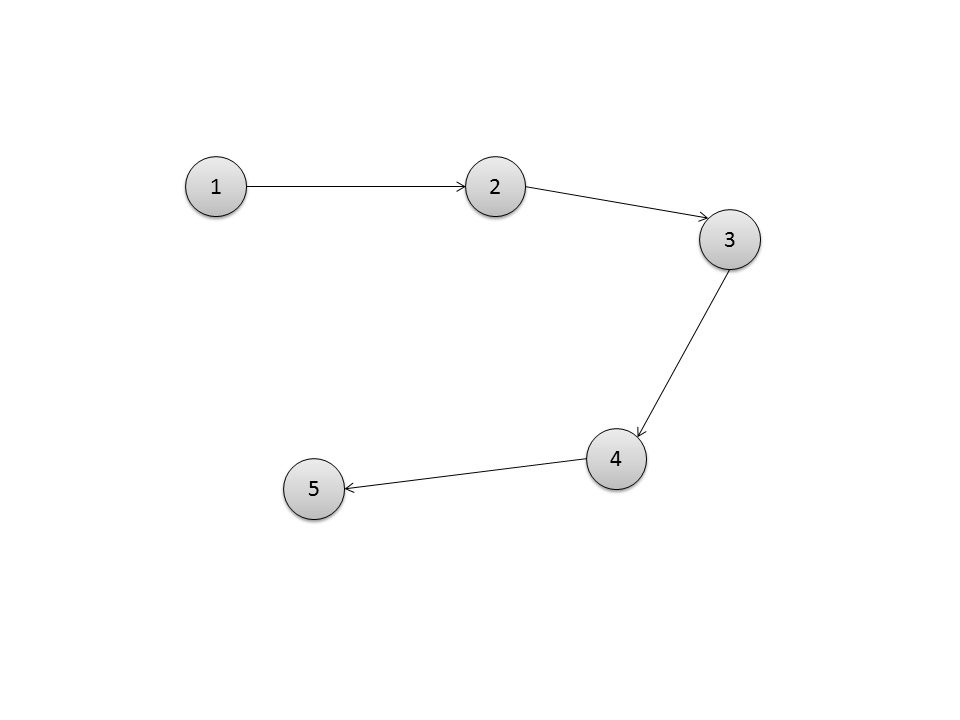
\includegraphics[width=0.7\textwidth]{img/cadena4.png}
	\caption{Nodos enlazados en una sola direcci\'on}
	\label{fig:Nodos enlazados en una sola direcci\'on}
\end{figure}
Nodos enlazados en una sola direcci\'on: consiste en un grafo formado por nodos que se conectan en una \'unica direcci\'on.
C\begin{figure}
	\centering
	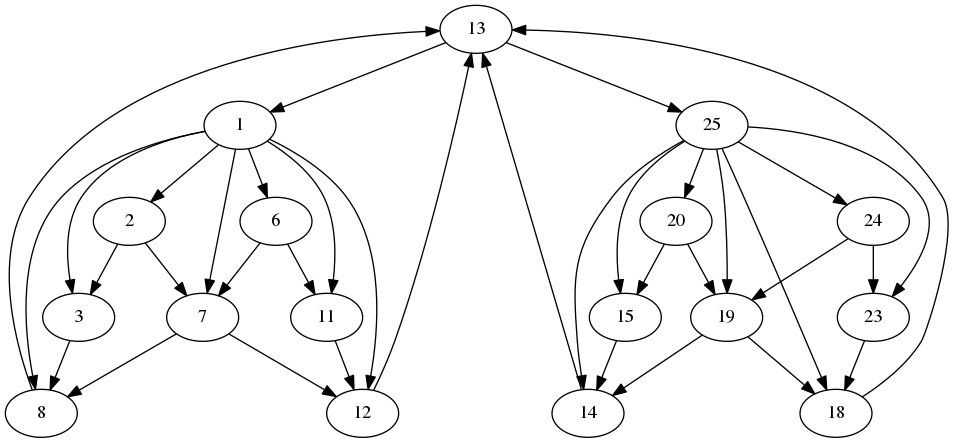
\includegraphics[width=0.7\textwidth]{img/links_salientes_25.png}
	\caption{Nodos con muchos links salientes}
	\label{fig:Nodos con muchos links salientes}
\end{figure}
Nodos con muchos links salientes: consiste en un grafo con dos nodos con muchos links salientes.
C\begin{figure}
	\centering
	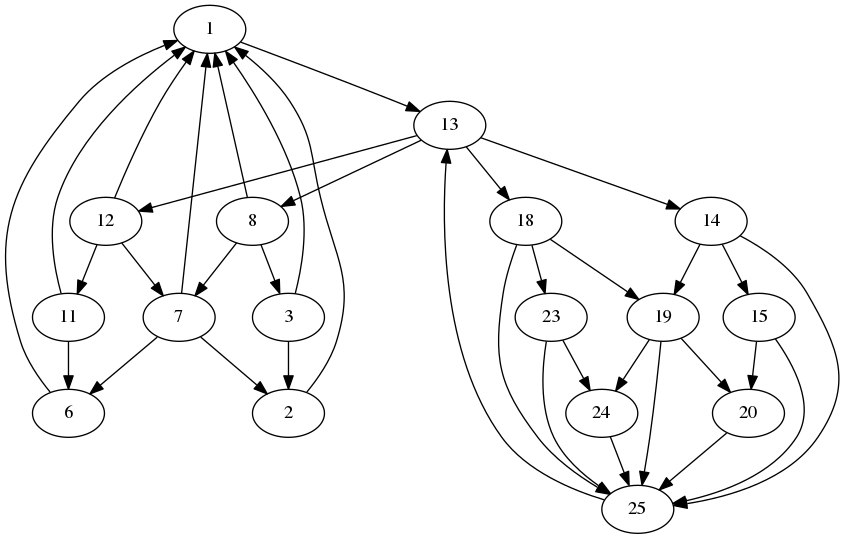
\includegraphics[width=0.7\textwidth]{img/links_entrantes_25.png}
	\caption{Nodos con muchos links entrantes}
	\label{fig:Nodos con muchos links entrantes}
\end{figure}
Nodos con muchos links entrantes: en este grafo hay dos nodos con muchos links entrantes.
C\begin{figure}
	\centering
	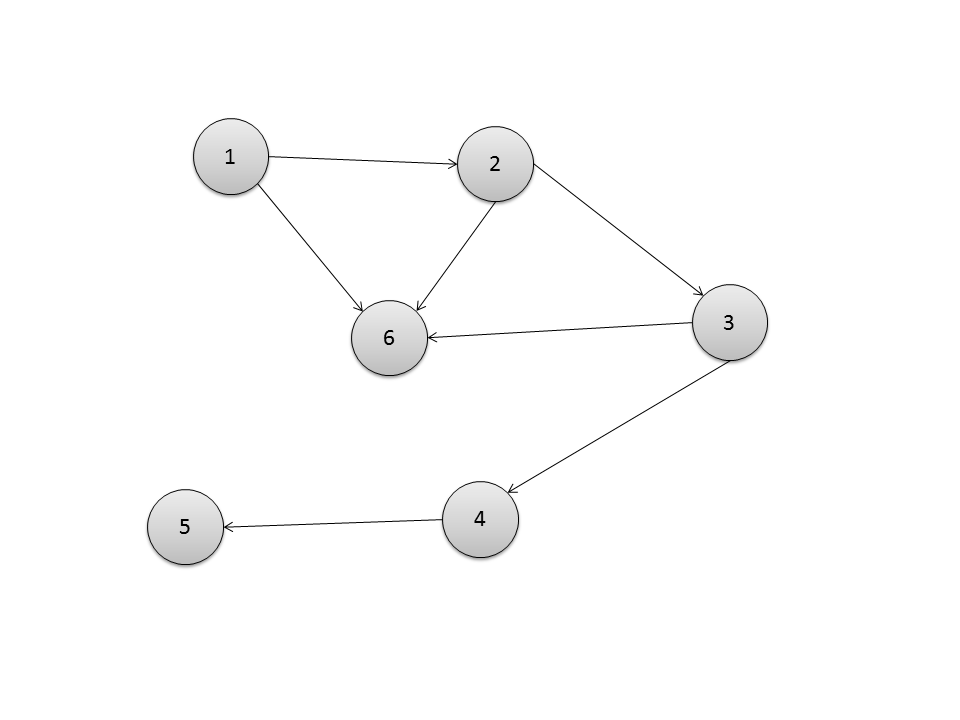
\includegraphics[width=0.7\textwidth]{img/Cadena6v1.png}
	\caption{Grafos sin links salientes}
	\label{fig:Grafos sin links salientes}
\end{figure}
Grafos sin links salientes: en este grafo hay dos nodos sin links salientes.
Para observar m\'as experimentos, dirigirse al ap\'endice ACA VA EL NUMERO DEL APENDICE.
\newpage

\section{Resultados}
\subsubsection*{Resultados obtenidos}

\newpage

\section{Discusión}
\subsubsection*{Discusión}


\newpage

\section{Conclusiones}
\subsubsection*{Conclusiones}

\newpage

\section{Apendices}
\subsubsection*{Demostraciones}
\providecommand{\abs}[1]{\lvert#1\rvert}
\providecommand{\norm}[1]{\lVert#1\rVert}

1) Justificar que:
\begin{displaymath}
A = p WD + ez^{t}
\end{displaymath}

Estudiemos como son los elementos de la matriz $A = p WD + ez^{t}$:

\begin{displaymath}
(p WD + ez^{t})_{ij} = p(W\,D)_{ij}+(ez^{t})_{ij} = p(\sum_{k=1}^{n}w_{ik}d_{kj}+1\,z^{t}_j)
\end{displaymath}

Como D es una matriz diagonal, los elementos distintos de cero únicamente pueden estar en la diagonal, con lo cual al hacer el producto se anulan todos los términos con $k\not=j$ y también aquellos términos donde $w_{ik}=0$ lo cual ocurre cuando $c_j=0$.

En consecuencia se puede reescribir:

\begin{displaymath}
(p WD + ez^{t})_{ij} = p(w_{ij}d_{jj}+z^{t}_j)
\end{displaymath}

Vamos a separar en casos para analizar los posibles valores que puede tomar el elemento (notar que por la definición de D, la condición $d_{jj}=0$ es equivalente a $c_j=0$):

caso 1: $w_{ij}=0, d_{jj}=0$ ($c_j=0$)$\Rightarrow(p WD + ez^{t})_{ij} =z_j^t=1/n$


caso 2: $w_{ij}=0, d_{jj}\not=0$ ($c_j\not=0$)$\Rightarrow(p WD + ez^{t})_{ij} =z_j^t=(1-p)/n$


caso 3: $w_{ij}=1, d_{jj}=0$ ($c_j=0$)$\Rightarrow(p WD + ez^{t})_{ij} =z_j^t=1/n$


caso 4: $w_{ij}=1, d_{jj}\not=0$ ($c_j\not=0$)$\Rightarrow(p WD + ez^{t})_{ij} =p/c_j+z_j^t=p/c_j+(1-p)/n$

Observando los casos 2 y 4 podemos observar que se pueden  unificar en una condición equivalente: $(p WD + ez^{t})_{ij} =w_{ij}p/c_j+z_j^t=p/c_j+(1-p)/n$

Uniendo todo lo anterior tenemos que:


\begin{equation}
 (p WD + ez^{t})_{ij} = \left\{
    \begin{array}{ll}
	 p\,w_{ij}/c_j+z_j^t=(1-p)/n+p/c_j & \mathrm{si\ } c_j \not= 0 \\
	 1/n & \mathrm{si\ } c_j=0
	 \end{array}
   \right.
\end{equation}
Pero precisamente esto coincide con la definición de los elementos de la matriz A. Luego $A = p WD + ez^{t}$.
%demostracion 2como se garantiza la aplicabilidad de EG

2) ¿Cómo se garantiza la aplicabilidad de la Eliminación Gaussiana? ¿La matriz $I-pWD$ está bien condicionada?¿Cómo influye el valor de p?

Primero veamos como se garantiza la aplicabilidad de Eliminación Gaussiana:

Sea $B=W\,D$,
\begin{displaymath}
B_{ij}=\sum_{k=1}^n w_{ik}d_{kj}
\end{displaymath}

Por la definición de D, cuando $k\not=j$, $d_{kj}=0$, por lo tanto se anulan los correspondientes términos de la sumatoria, quedando:

\begin{displaymath}
B_{ij}=w_{ij}d_{jj}
\end{displaymath}

También sabemos por la definición de W que $w_{jj}=0$ (porque no se consideran los autolinks), así que podemos deducir que los elementos de la diagonal van a ser iguales a cero, luego:

\begin{equation}
 B_{ij} = \left\{
    \begin{array}{ll}
	 0 & \mathrm{si\ } i=j \\
	 1/c_j & \mathrm{si\ } i\not=j,  w_{ij}\not=0
	 \end{array}
   \right.
\end{equation}

Y por lo tanto:

\begin{equation}
(I-p B)_{ij} = \left\{
    \begin{array}{ll}
	 1 & \mathrm{si\ } i=j \\
	 -p/c_j & \mathrm{si\ } i\not=j
	 \end{array}
   \right.
\end{equation}

La matriz B tiene la particularidad de que la suma de los elementos de cada columna es igual a 1, ya que en cada columna hay $c_j$ elementos de valor $1/c_j$. Por lo tanto en $I-p B$ la suma de los elementos de cada columna es $1+c_j\, p/c_j$ con $|c_j\, p/c_j|<1$ porque $0<p<1$. De esto se desprende que $(I-p B)^t$ es estrictamente diagonal dominante y como se probó en la teórica esto implica que sea no singular. Además, si una matriz es e.d.d. cada una de sus submatrices principales es e.d.d. y entonces todas ellas son no singulares. Por otra parte se puede probar que si una matriz tiene inversa, su traspuesta tiene inversa (ejercicio 23 c), Práctica 1). Luego podemos afirmar que $(I-p B)$ es no singular y que todas sus submatrices principales también son no singulares, esto garantiza que $(I-p B)$ tiene descomposición $LU$ que es equivalente a decir que puede realizarse la Eliminación Gaussiana sin necesidad de pivoteo en ninguno de los pasos del proceso.

Con respecto al condicionamiento de la matriz, se puede aplicar una propiedad demostrada en la práctica (ejercicio 21, Práctica 2) la cual afirma que: Dada $M \in$ $\mathbb{R}^{nxn}$ tal que $||M||<1$, $I$ la matriz identidad de $\mathbb{R}^{nxn}$ 
i $||.||$ norma inducida por una norma vectorial: $I+M$ es inversible y $||(I+R)^{-1}||\leq 1/(1-||M||)$.\\

De lo que vimos arriba acerca del formato de las matrices tratadas en el TP, también deducimos que tomando $||.||_1$, $M = -pWD$ estamos en las hipótesis del ejercicio, porque:

\begin{displaymath}
||-pWD||_1=||pWD||_1=|p|||WD||_1=p*c_j*1/c_j=p.
\end{displaymath}
Y como $p<1$, implica que:
\begin{displaymath}
||(I-pWD)^{-1}||_1\leq 1/(1-||I-pWD||_1)
\end{displaymath}
Si calculamos el número de condición,
\begin{displaymath}
K=||I-pWD||||(I-pWD)^{-1}||\leq (1+p) (1/(1-||pWD||)=(1+p) (1/(1-p||WD||)=(1+p)/(1-p)
\end{displaymath}

Cuanto menor sea $p$ mas cerca de 1 estará el número de condición, lo cual es lógico porque la matriz se parecerá más a I que tiene la característica de tener sus columnas ortogonales. A medida que crece $p$ va aumentando el valor de $K$ tendiendo a infinito si $p$ tiende a 1. en el gráfico \ref{K(p)} se puede ver la relación entre el número de condición y el valor de $p$. Con un ejemplo se puede ver que con un valor relativamente cercano a 1 (0.9) el número de condición sigue siendo aceptable, y recién con valores mayores se puede decir que aumenta rápidamente.
Supongamos p = 0.9:
$K\leq (1.9/0.1)=19$.

Para p=0.99: 
$K\leq (1.99/0.01)=199$. 

\begin{figure}[H]
  \centering
    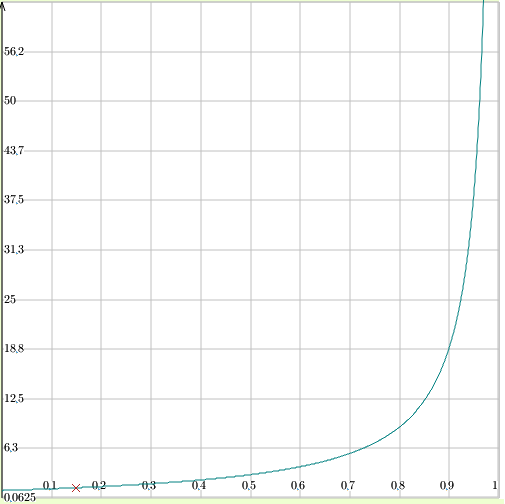
\includegraphics[width=0.7\textwidth]{img/K_tp1.png}
  \caption{K en función de p}
  \label{fig:K(p)}
\end{figure}


\subsubsection*{Tests Cualitativos}



\begin{figure}[H]
  \centering
    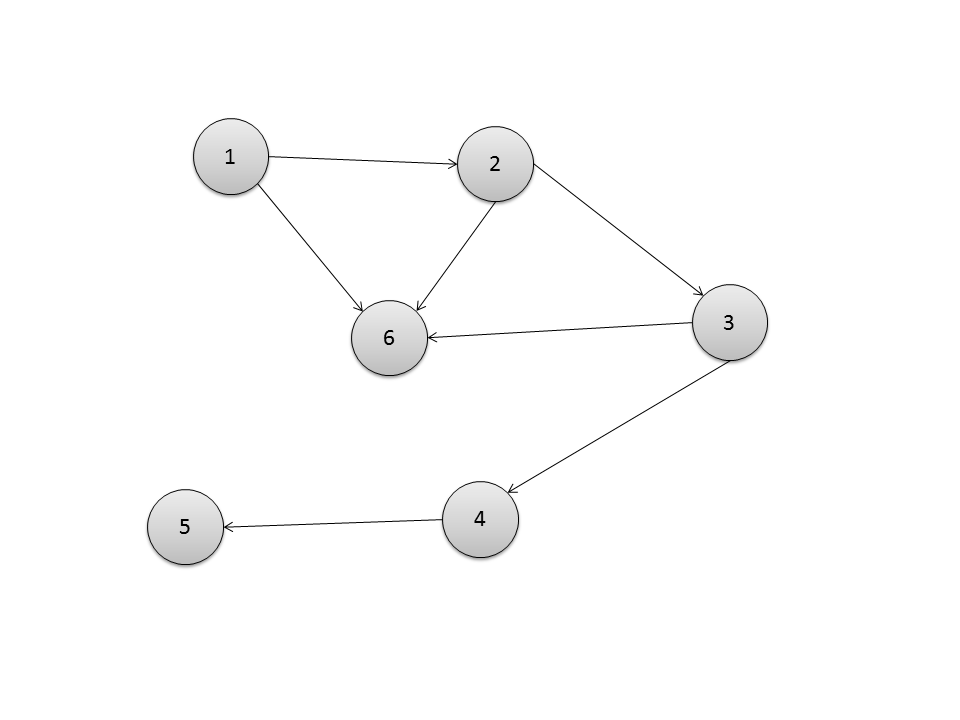
\includegraphics[width=0.7\textwidth]{img/Cadena6v1.png}
  \caption{Cadena con nodo central (caso 1)}
  \label{fig: Cadena con nodo central (caso 1)}
\end{figure}


\begin{figure}[H]
  \centering
    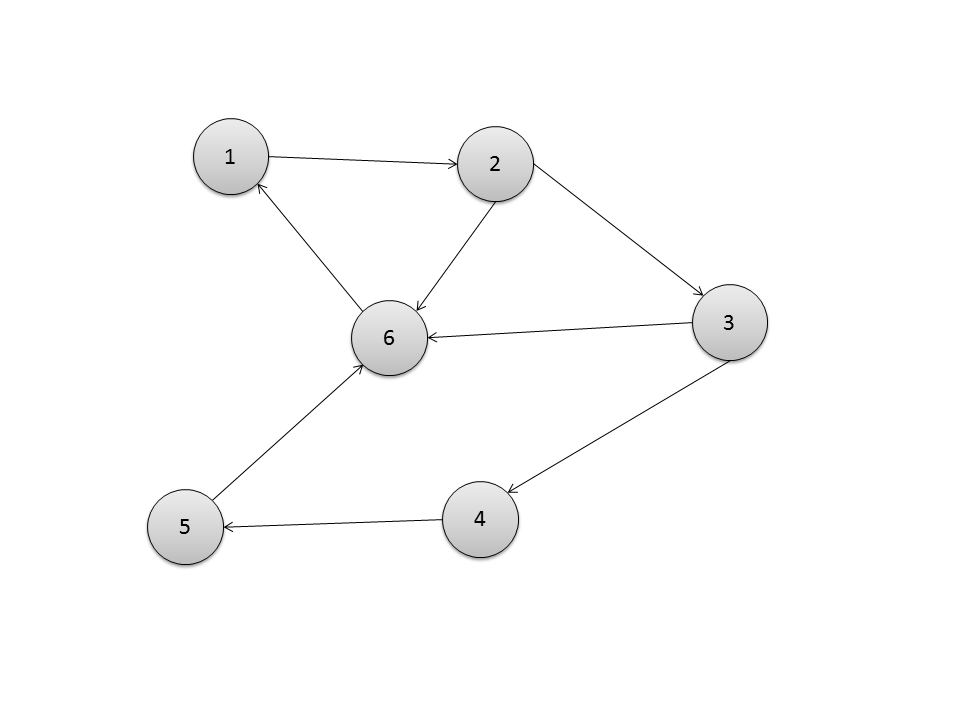
\includegraphics[width=0.7\textwidth]{img/Cadena6v3.png}
  \caption{Cadena con nodo central (caso 3)}
  \label{fig: Cadena con nodo central, con ciclo}
\end{figure}


\begin{figure}[H]
  \centering
    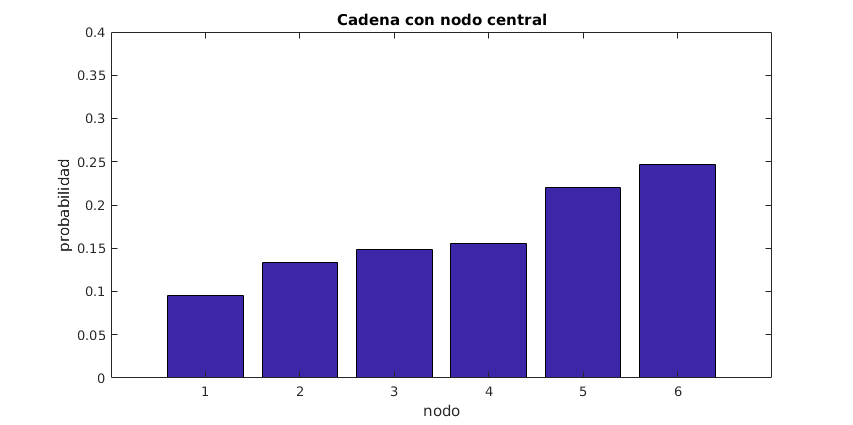
\includegraphics[width=0.7\textwidth]{img/cadena6v1.png}
  \caption{Cadena con nodo central (caso 1)}
  \label{fig: Cadena con nodo central (caso 1)}
\end{figure}


\begin{figure}[H]
  \centering
    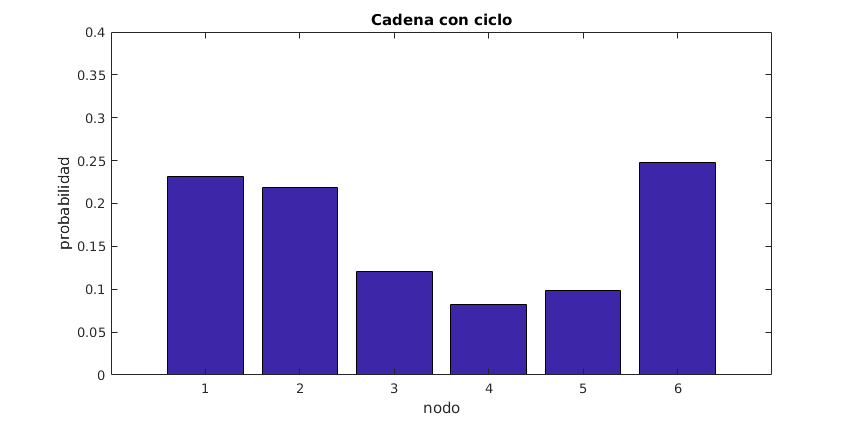
\includegraphics[width=0.7\textwidth]{img/cadena6v3.png}
  \caption{Cadena con nodo central (caso 3)}
  \label{fig: Cadena con nodo central, con ciclo}
\end{figure}

\begin{figure}[H]
	\centering
	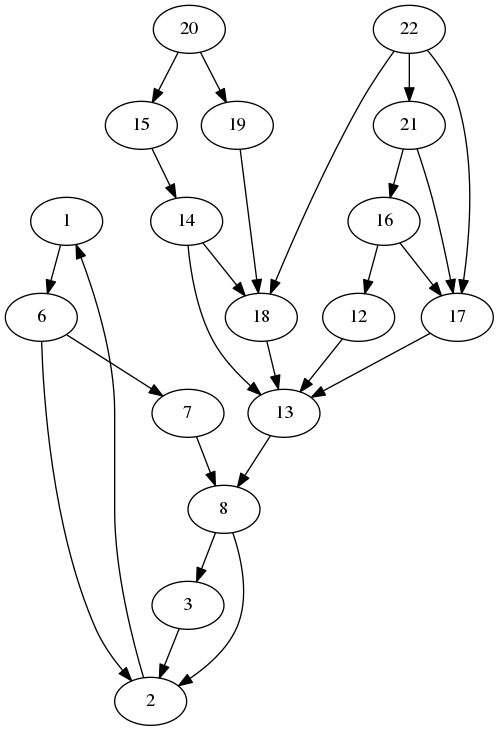
\includegraphics[width=0.7\textwidth]{img/links_a_ciclo_25.png}
	\caption{Grafo con ciclo}
	\label{fig: Grafo con ciclo}
\end{figure}

\begin{figure}[H]
	\centering
	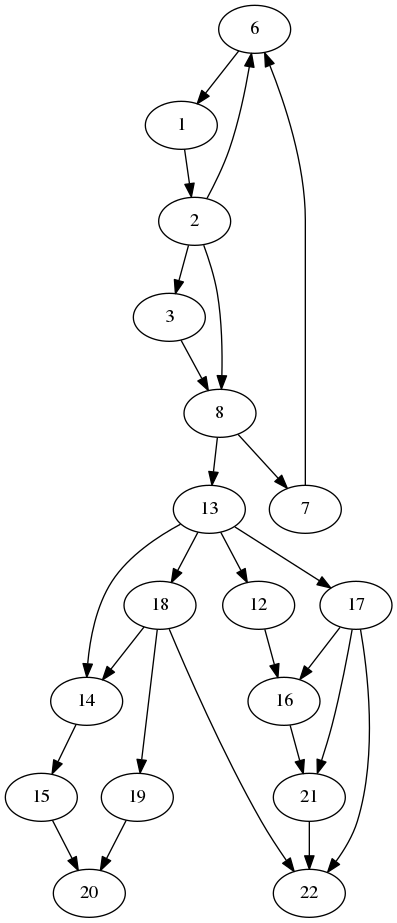
\includegraphics[width=0.7\textwidth]{img/links_a_ciclo_al_reves_25.png}
	\caption{Grafo con ciclo al rev\'es}
	\label{fig: Grafo con ciclo al rev\'es}
\end{figure}

\begin{figure}[H]
	\centering
	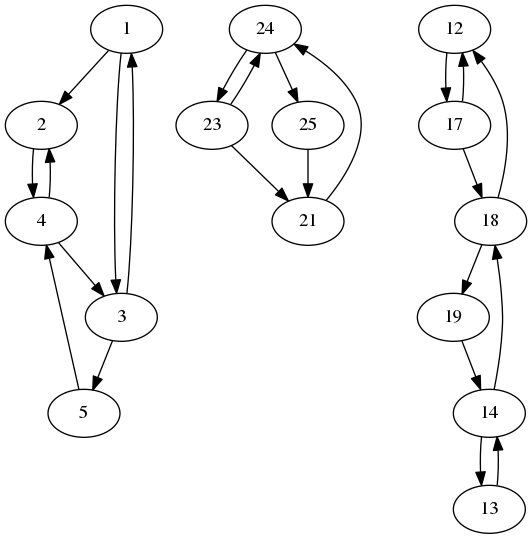
\includegraphics[width=0.7\textwidth]{img/links_grafos_separados_25.png}
	\caption{Grafos separados}
	\label{fig: Grafos separados}
\end{figure}

\begin{table}[H]
\centering
	\begin{tabular}{|c|c|c|c|}
		\hline
		Nodo & Probabilidad & Nodo & Probabilidad \\ \hline
		4    & 0.092437     & 1    & 0.0372149    \\
		24   & 0.0815273    & 5    & 0.0372149    \\
		14   & 0.0768427    & 6    & 0.0117647    \\
		18   & 0.0677026    & 7    & 0.0117647    \\
		21   & 0.0650155    & 8    & 0.0117647    \\
		12   & 0.0640465    & 9    & 0.0117647    \\
		2    & 0.0636255    & 10   & 0.0117647    \\
		3    & 0.0636255    & 11   & 0.0117647    \\
		17   & 0.0630019    & 15   & 0.0117647    \\
		23   & 0.0443756    & 16   & 0.0117647    \\
		25   & 0.0443756    & 20   & 0.0117647    \\
		13   & 0.0425018    & 22   & 0.0117647    \\
		19   & 0.0388457    & ~    & ~            \\ \hline
	\end{tabular}
\caption {Tabla de resultados}
\end{table}

\begin{table}[H]
\centering
	\begin{tabular}{|c|c|c|c|}
		\hline
		Nodo & Probabilidad & Nodo & Probabilidad \\ \hline
		2    & 0.155359     & 19   & 0.0150538    \\
		1    & 0.13504      & 21   & 0.0136201    \\
		8    & 0.122903     & 4    & 0.0107527    \\
		6    & 0.118784     & 5    & 0.0107527    \\
		13   & 0.0819211    & 9    & 0.0107527    \\
		3    & 0.0599138    & 10   & 0.0107527    \\
		7    & 0.0582664    & 11   & 0.0107527    \\
		18   & 0.0347814    & 20   & 0.0107527    \\
		17   & 0.0255484    & 22   & 0.0107527    \\
		14   & 0.0227957    & 23   & 0.0107527    \\
		12   & 0.017233     & 24   & 0.0107527    \\
		16   & 0.0162007    & 25   & 0.0107527    \\
		15   & 0.0150538    & ~    & ~            \\ \hline
	\end{tabular}
\caption{Tabla de resultados links a ciclo}
\end{table}

\begin{table}[H]
\centering
	\begin{tabular}{|c|c|c|c|}
		\hline
		Nodo & Probabilidad & Nodo & Probabilidad \\ \hline
		22   & 0.0795721    & 12   & 0.0262073    \\
		2    & 0.0783998    & 17   & 0.0262073    \\
		1    & 0.0764254    & 18   & 0.0262073    \\
		6    & 0.0739574    & 19   & 0.0242481    \\
		20   & 0.0717109    & 4    & 0.0172595    \\
		8    & 0.068699     & 5    & 0.0172595    \\
		21   & 0.0604193    & 9    & 0.0172595    \\
		16   & 0.0452139    & 10   & 0.0172595    \\
		7    & 0.0447391    & 11   & 0.0172595    \\
		13   & 0.0447391    & 23   & 0.0172595    \\
		15   & 0.0438162    & 24   & 0.0172595    \\
		3    & 0.0381661    & 25   & 0.0172595    \\
		14   & 0.0331959    & ~    & ~            \\ \hline
	\end{tabular}
\caption{Tabla de resultados links a ciclo al reves}
\end{table}


\section{Referencias}
\begin{thebibliography}{9}

\bibitem{navegante} 

http://www-2.dc.uba.ar/materias/metnum/dnload/2018\_C1/tp1/Enunciado\_TP1.pdf

\bibitem{burden} 
Richard L. Burden, J. Douglas Faires
\textit{Numerical Analysis}. (Ingles) 
[\textit{An\'alisis num\'erico}]. 
International Thomson, :358-362, 9th Edition, 2010.

\end{thebibliography}


\newpage
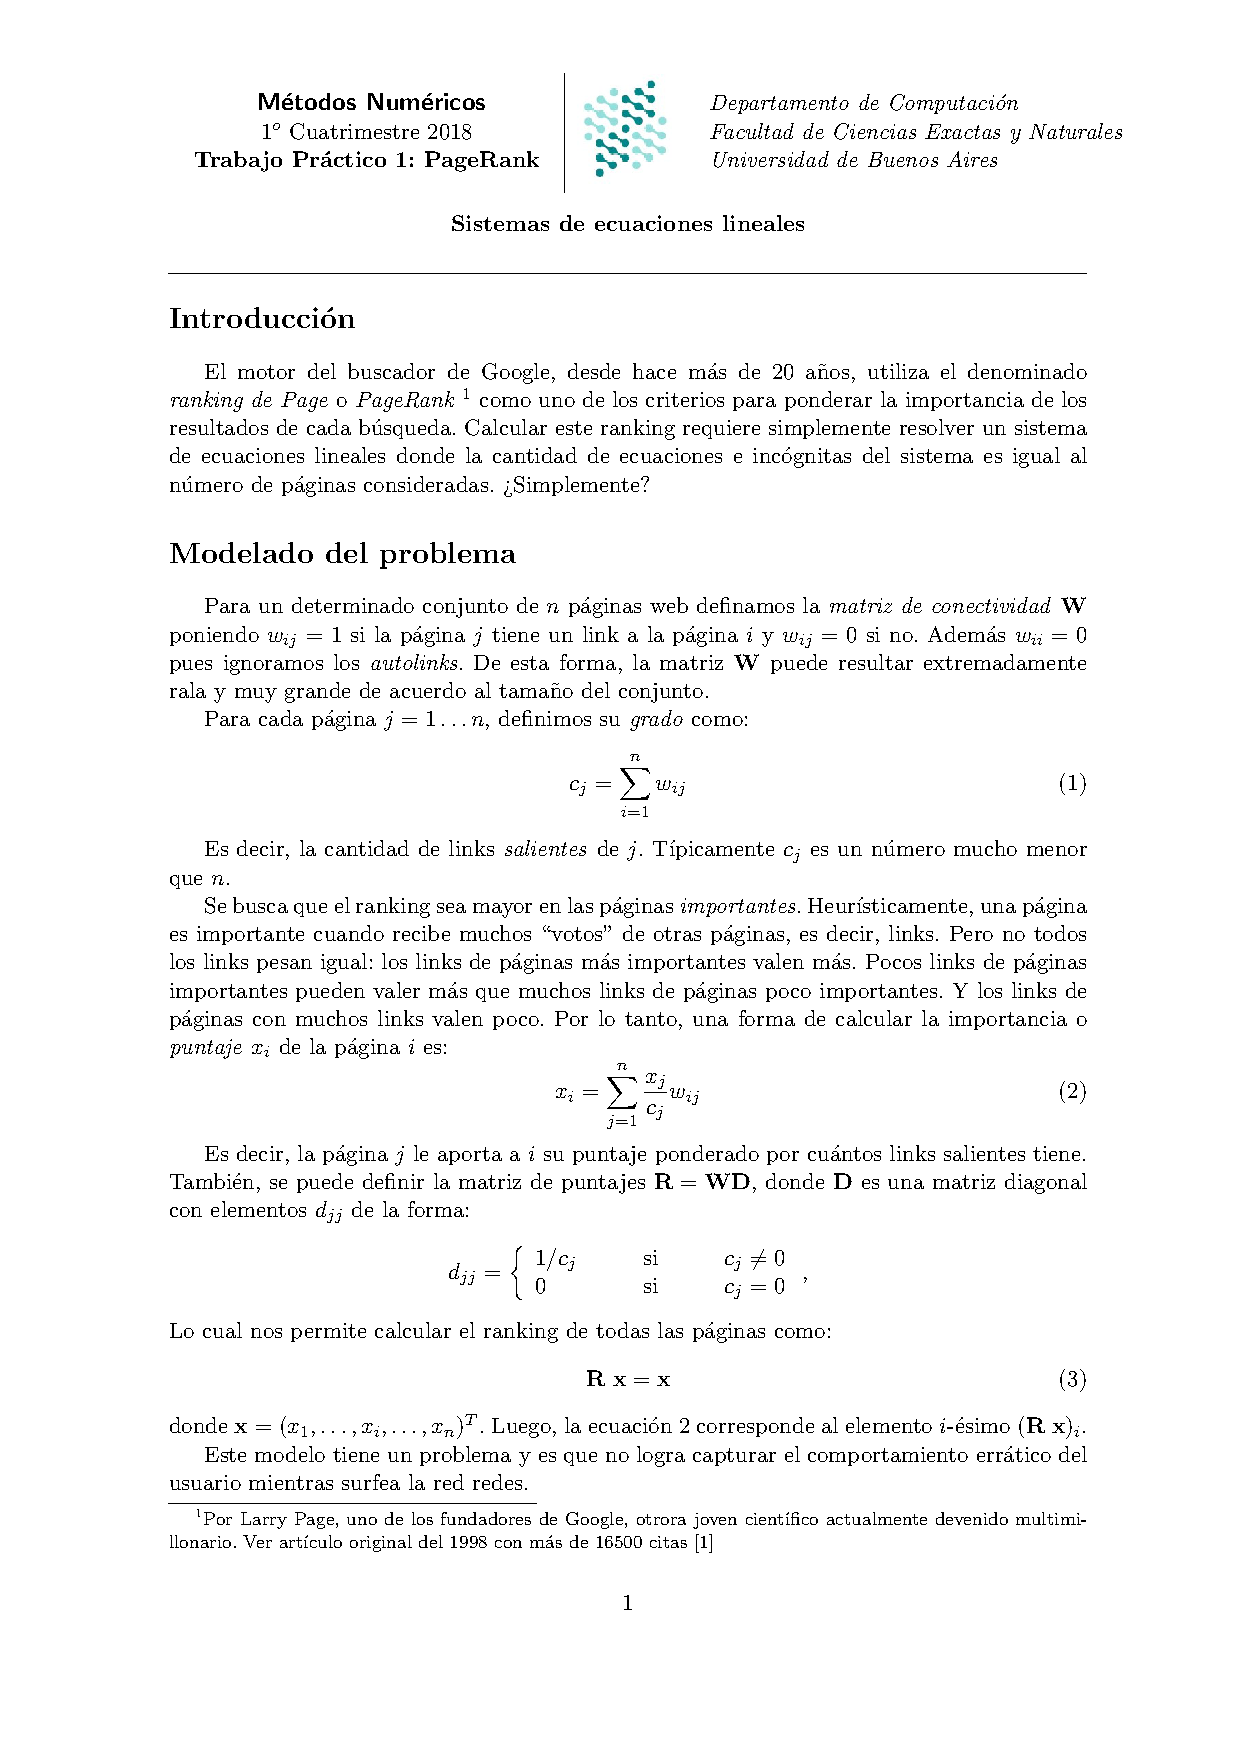
\includepdf[pages=-]{Enunciado.pdf}


\documentclass[a4paper]{article}

\usepackage[spanish]{babel} % Le indicamos a LaTeX que vamos a escribir en español.
\usepackage[utf8]{inputenc} % Permite utilizar tildes y eñes normalmente
\begin{document}

Justificar que:
\begin{displaymath}
A = p WD + ez^{t}
\end{displaymath}

Estudiemos como son los elementos de la matriz $A = p WD + ez^{t}$:

\begin{displaymath}
(p WD + ez^{t})_{ij} = p(W\,D)_{ij}+(ez^{t})_{ij} = p(\sum_{k=1}^{n}w_{ik}d_{kj}+1\,z^{t})
\end{displaymath}

Como D es una matriz diagonal, los elementos distintos de cero únicamente pueden estar en la diagonal, con lo cual al hacer el producto se anulan todos los términos con $k\not=j$ y también aquellos términos donde $w_{ik}=0$ lo cual ocurre cuando $c_j=0$.

En consecuencia se puede reescribir:

\begin{displaymath}
(p WD + ez^{t})_{ij} = p(w_{ij}d_{jj}+z^{t})
\end{displaymath}

Vamos a separar en casos para analizar los posibles valores que puede tomar el elemento (notar que por la definición de D, la condición $d_{jj}=0$ es equivalente a $c_j=0$):

caso 1: $w_{ij}=0, d_{jj}=0$ ($c_j=0$)$\Rightarrow(p WD + ez^{t})_{ij} =z_j^t=1/n$


caso 2: $w_{ij}=0, d_{jj}\not=0$ ($c_j\not=0$)$\Rightarrow(p WD + ez^{t})_{ij} =z_j^t=(1-p)/n$


caso 3: $w_{ij}=1, d_{jj}=0$ ($c_j=0$)$\Rightarrow(p WD + ez^{t})_{ij} =z_j^t=1/n$


caso 4: $w_{ij}=1, d_{jj}\not=0$ ($c_j\not=0$)$\Rightarrow(p WD + ez^{t})_{ij} =p/c_j+z_j^t=p/c_j+(1-p)/n$

Observando los casos 2 y 4 podemos observar que se pueden  unificar en una condición equivalente: $(p WD + ez^{t})_{ij} =w_{ij}p/c_j+z_j^t=p/c_j+(1-p)/n$

Uniendo todo lo anterior tenemos que:


\begin{equation}
 (p WD + ez^{t})_{ij} = \left\{
    \begin{array}{ll}
	 p\,w_{ij}/c_j+z_j^t=(1-p)/n+p/c_j & \mathrm{si\ } c_j \not= 0 \\
	 1/n & \mathrm{si\ } c_j=0
	 \end{array}
   \right.
\end{equation}
Pero precisamente esto coincide con la definición de los elementos de la matriz A. Luego $A = p WD + ez^{t}$.
%demostracion 2como se garantiza la aplicabilidad de EG

¿Cómo se garantiza la aplicabilidad de la Eliminación Gaussiana? ¿La matriz $I-pWD$ está bien condicionada?¿Cómo influye el valor de p?

Sea $B=W\,D$,
\begin{displaymath}
B_{ij}=\sum_{k=1}^n w_{ik}d_{kj}
\end{displaymath}

Por la definición de D, cuando $k\not=j$, $d_{kj}=0$, por lo tanto se anulan los correspondientes términos de la sumatoria, quedando:

\begin{displaymath}
B_{ij}=w_{ij}d_{jj}
\end{displaymath}

También sabemos por la definición de W que $w_{jj}=0$ (porque no se consideran los autolinks), así que podemos deducir que los elementos de la diagonal van a ser iguales a cero, luego:

\begin{equation}
 B_{ij} = \left\{
    \begin{array}{ll}
	 0 & \mathrm{si\ } i=j \\
	 1/c_j & \mathrm{si\ } i\not=j,  w_{ij}\not=0
	 \end{array}
   \right.
\end{equation}

Y por lo tanto:

\begin{equation}
(I-p B)_{ij} = \left\{
    \begin{array}{ll}
	 1 & \mathrm{si\ } i=j \\
	 -p/c_j & \mathrm{si\ } i\not=j
	 \end{array}
   \right.
\end{equation}

La matriz B tiene la particularidad de que la suma de los elementos de cada columna es igual a 1, ya que en cada columna hay $c_j$ elementos de valor $1/c_j$. Por lo tanto en $I-p B$ la suma de los elementos de cada columna es $1+c_j\, p/c_j$ con $|c_j\, p/c_j|<1$ porque $0<p<1$. De esto se desprende que $(I-p B)^t$ es estrictamente diagonal dominante y como se probó en la teórica esto implica que sea no singular. Además, si una matriz es e.d.d. cada una de sus submatrices principales es e.d.d. y entonces todas son no singulares. Por otra parte se puede probar que si una matriz tiene inversa, su traspuesta tiene inversa. Luego podemos afirmar que $(I-p B)$ es no singular y que todas sus submatrices principales también son no singulares, luego $(I-p B)$ tiene descomposición $LU$ que es equivalente a decir que puede realizarse la Eliminación Gaussiana sin que aparezca un cero en la diagonal en ninguno de los pasos del proceso.

\end{document}


\newpage

\section{Referencias}
\begin{thebibliography}{9}

\bibitem{navegante} 

http://www-2.dc.uba.ar/materias/metnum/dnload/2018\_C1/tp1/Enunciado\_TP1.pdf

\bibitem{burden} 
Richard L. Burden, J. Douglas Faires
\textit{Numerical Analysis}. (Ingles) 
[\textit{An\'alisis num\'erico}]. 
International Thomson, :358-362, 9th Edition, 2010.

\end{thebibliography}


\end{document}

